\subsubsubsubsection{Application}
\begin{figure}[h]
\centering
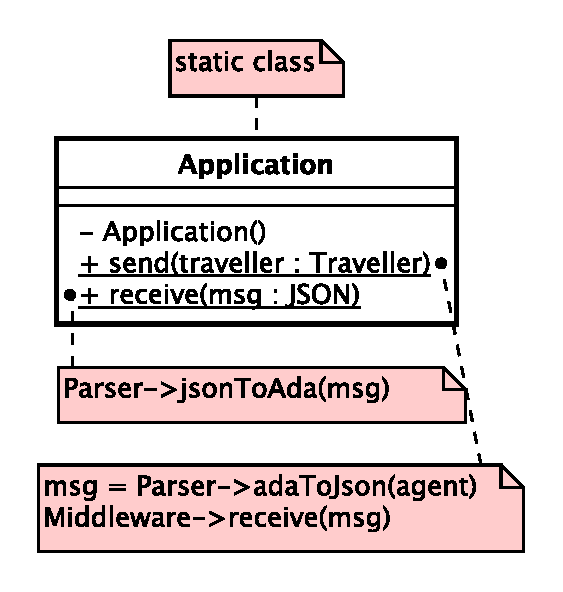
\includegraphics[scale=0.6,keepaspectratio]{images/solution/app/backend/application.eps}
\caption{\pInterface::Application}
\label{fig:sd-app-application}
\end{figure}
\FloatBarrier
\begin{itemize}
  \item \textbf{\descr} \\
    Lightweight interface to communicate with the middleware layer.
    It is a static class because it is composed of only static methods.
  \item \textbf{\ops}
  \begin{itemize}
   \item \texttt{Application()} \\
   Private and unique constructor because \texttt{Application} provides 
   only static methods so there are no reasons a client creates instances 
   of \texttt{Application}.
    \item[+] \texttt{\underline{send(agent: MoveableAgent)}} \\
    Sends messages to the middleware layer. Before sending the message to the
    middleware it converts the entity into a JSON message using the parser.
    \item[+] \texttt{\underline{receive(msg: JSON)}} \\
    Receives a JSON messae from the middleware layer. It invokes the parser 
    passing the message as parameter.
  \end{itemize}
\end{itemize}
